\section{Method Overview}
\label{sec:method}
\subsection{Problem Statement}
Given series of point sets which record the same group of rigid indoor objects with different layout. We intend to samutaneously partition the point sets into objects and align the points of same object to recover layouts for corresponding object. Figure~\ref{fig:syn-data} shows an example of input point clouds set.
\subsection{Basic Formulation}
To formulate the relation between the unknown object set and the input point clouds. We come up with a generation model as follows:
\begin{equation}
\label{equ:model}
P(v_{mi})=\sum^{K_n}_{k=1}p_kN(v_{mi}|\phi_{mn}(x_k),\Sigma_k)
\end{equation}
which means,
The observed point clouds are generated by $N$ object model. 
Each object model is represented by a gaussian mixture model with $K_n$ centroids.
Our goal is to maximize the probability of the expected compelete-data log-likelihood. 
The object function can be written as:
\begin{equation}
\label{equ:obj0}
\Theta=\arg\max{\sum_ZP(Z|V,\Theta)\ln{P(V,Z;\Theta)}}
\end{equation}
in which:
$$\Theta=\{\{p_k,x_k,\Sigma_k\}_{k=1}^{\sum{K_n}},\{\phi_{mn}\}_{m=1,n=1}^{MN}\}$$
is the parameters of the generation model.\\
$p_n$ is the prior probability that the point is generated by the n-th object.\\
$p_k$ is the weight of the k-th Gaussian.\\
$x_k$ is the center of the k-th Gaussian.\\
$\Sigma_k$ is the standard deviation of the k-th Gaussian.\\
There are $\sum{K_n}$ Gaussian model in total and among them, $K_n$ Gaussian models belongs to object $n$.\\
$V$ is the M input point clouds.\\
$v_{mi}$ is the i-th point of the m-th point cloud.\\
$Z$ is a latent variable set defined as:\\
$$Z=\{z_{ij}|j=1...M,i=1...N_j\}$$
among which if $z_{ij}=k(k=1...\sum{K_n})$ assign the observation of $\phi_{mn}(v_{mi})$ to the k-th component of Gaussian mixture model.Such formulation can be seen as an extention of joint registration formulation in \cite{Evangelidis2014}, upon which we add several gaussian mixture model together to express a group of objects. By solving this new problem we simutaneously solve  the object co-segmentation of given observation.
\subsection{Bilateral Formulation}
When considering features, we can develop it into a bilateral GMM formulation.
\begin{equation}
P(v_{mi},f_{mi})=\sum^{K_n}_{k=1}p_kN(v_{mi}|\phi_{mn}(xv_k),\sigma v_k)N(f_{mi}|xf_k,\sigma v_f)
\end{equation}
we measure the feature difference by a gaussian with diagnal $\Sigma$.
\subsection{Interaction Design}
Unfortunately, there are serveral parameters that can not be easily initialized in our formulation . In this subsection we first introduce our design of interaction, which is intuitive for users to input the semantic prior this way. We then explain how we can easily initlialize those parameters for our optimization based on the manual input.\\
As demonstrated in Figure~\ref{fig:interact}, we let user choose one of the point sets and placing and editing boxes in it to indicate the layout for this point set. From this, we can easily initialize the total number of objects $N$ and determine $\{K_n\}$ which is the numbers of Gaussian mixture models used to represent each object.
\begin{figure}[htb]
	\centering
	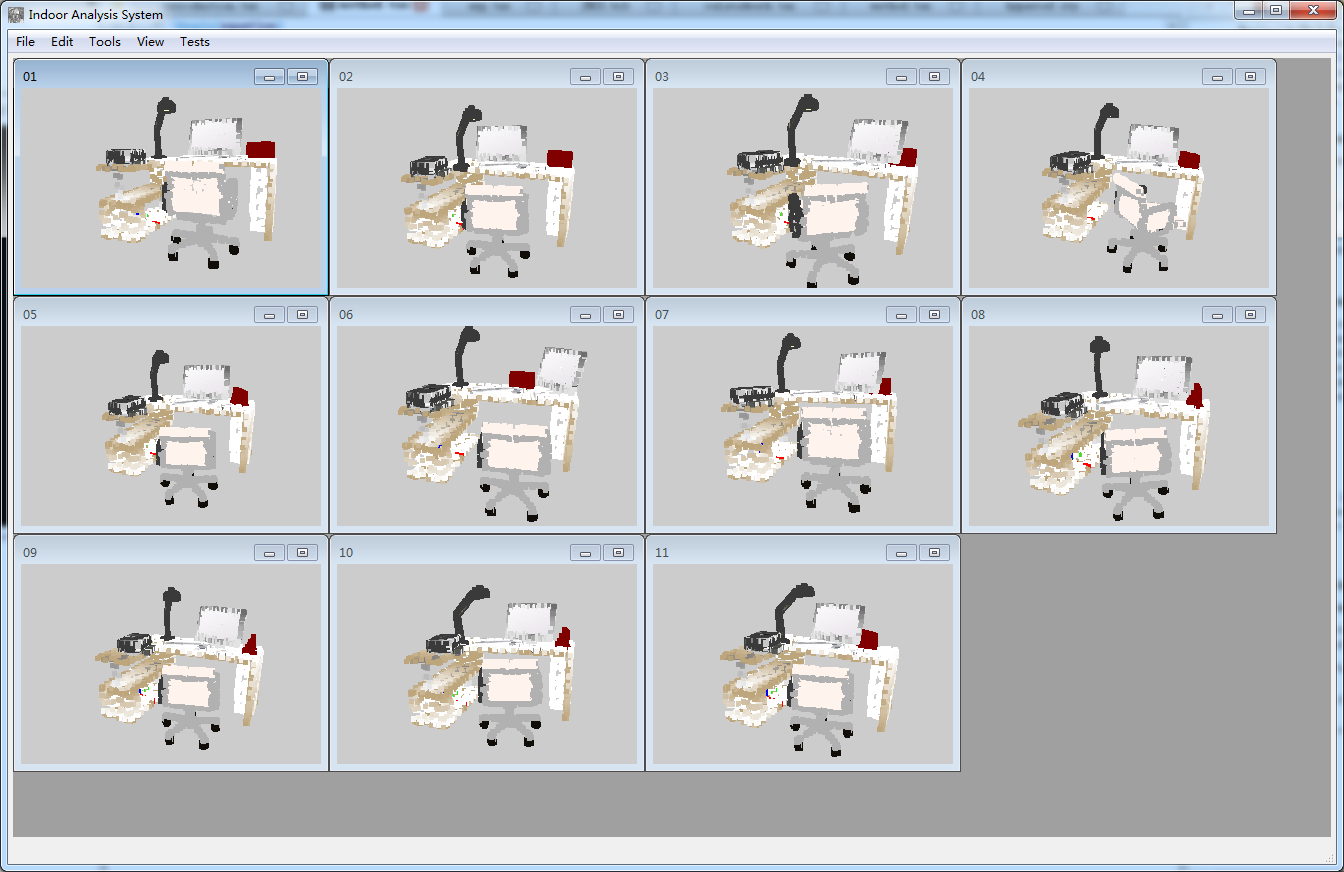
\includegraphics[width=.3\linewidth]{images/interact01.png}
	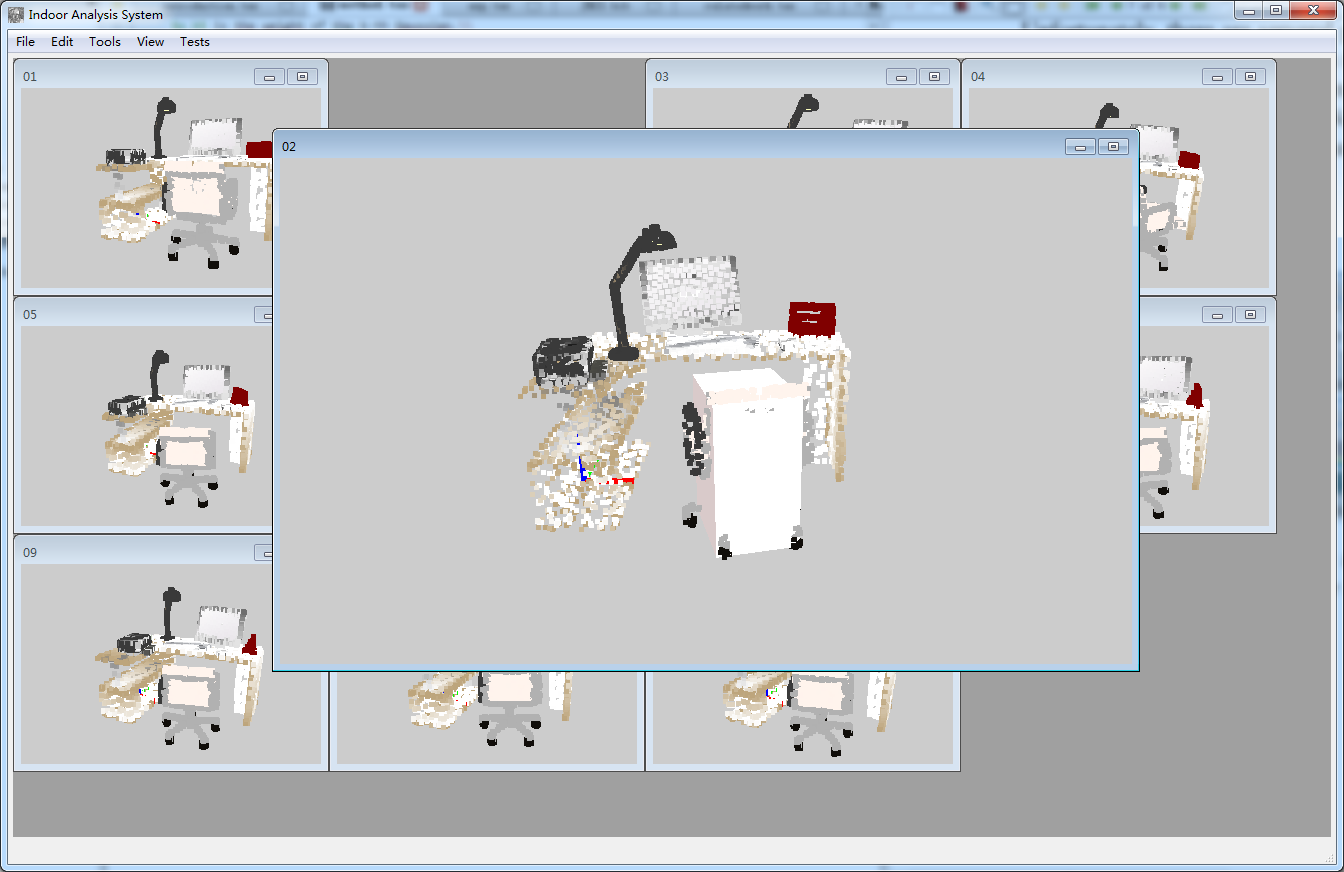
\includegraphics[width=.3\linewidth]{images/interact02.png}
	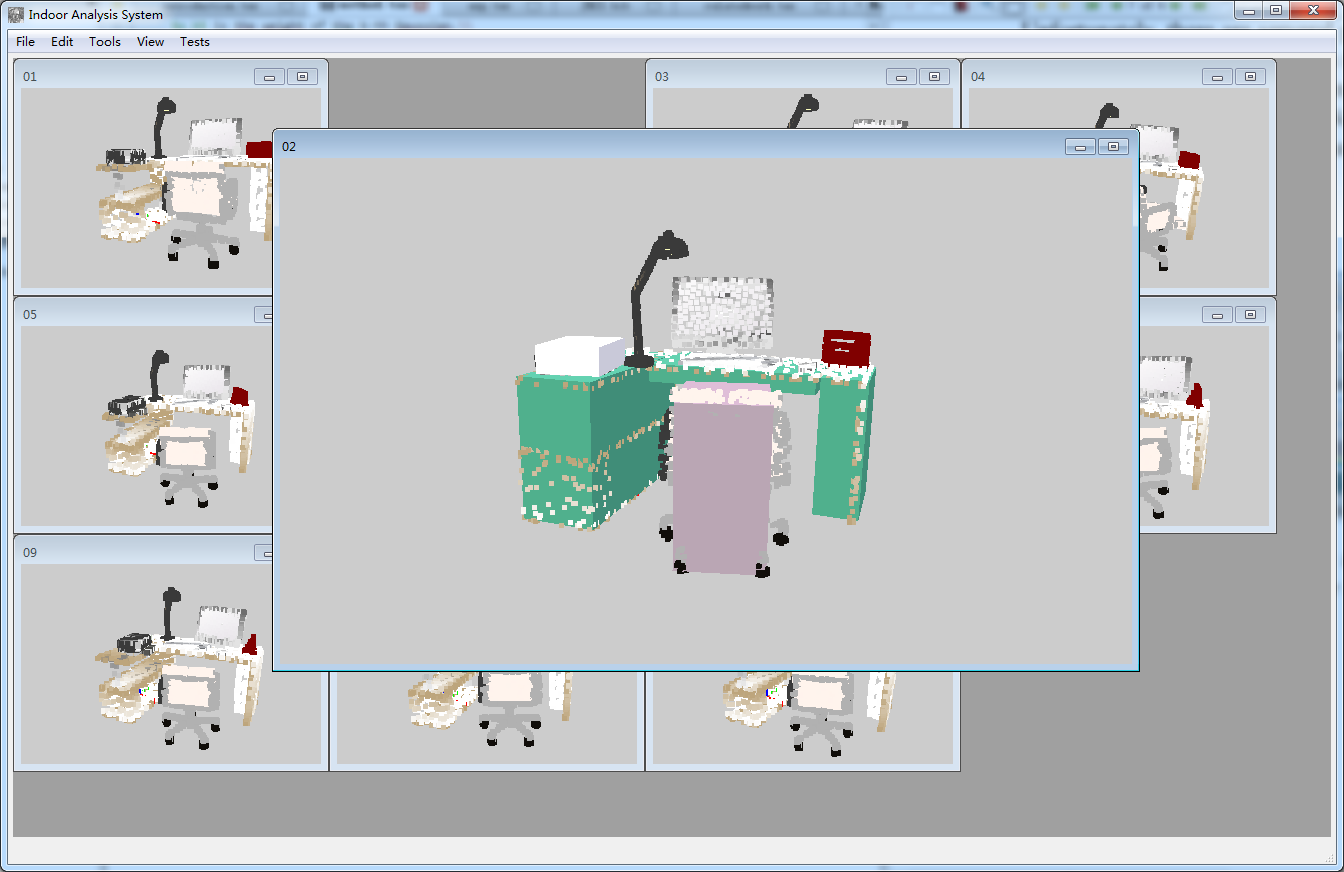
\includegraphics[width=.3\linewidth]{images/interact03.png}
	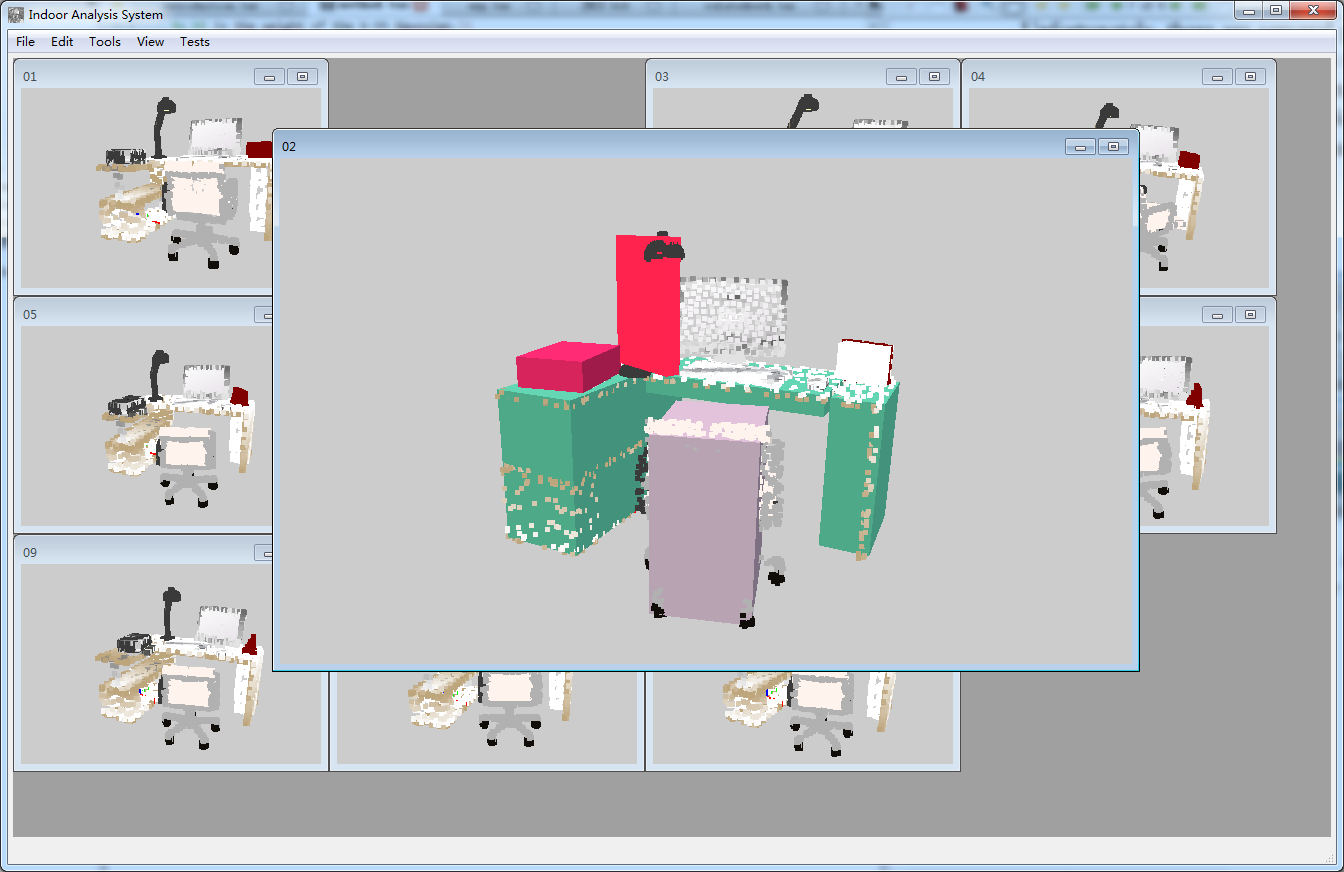
\includegraphics[width=.3\linewidth]{images/interact04.png}
	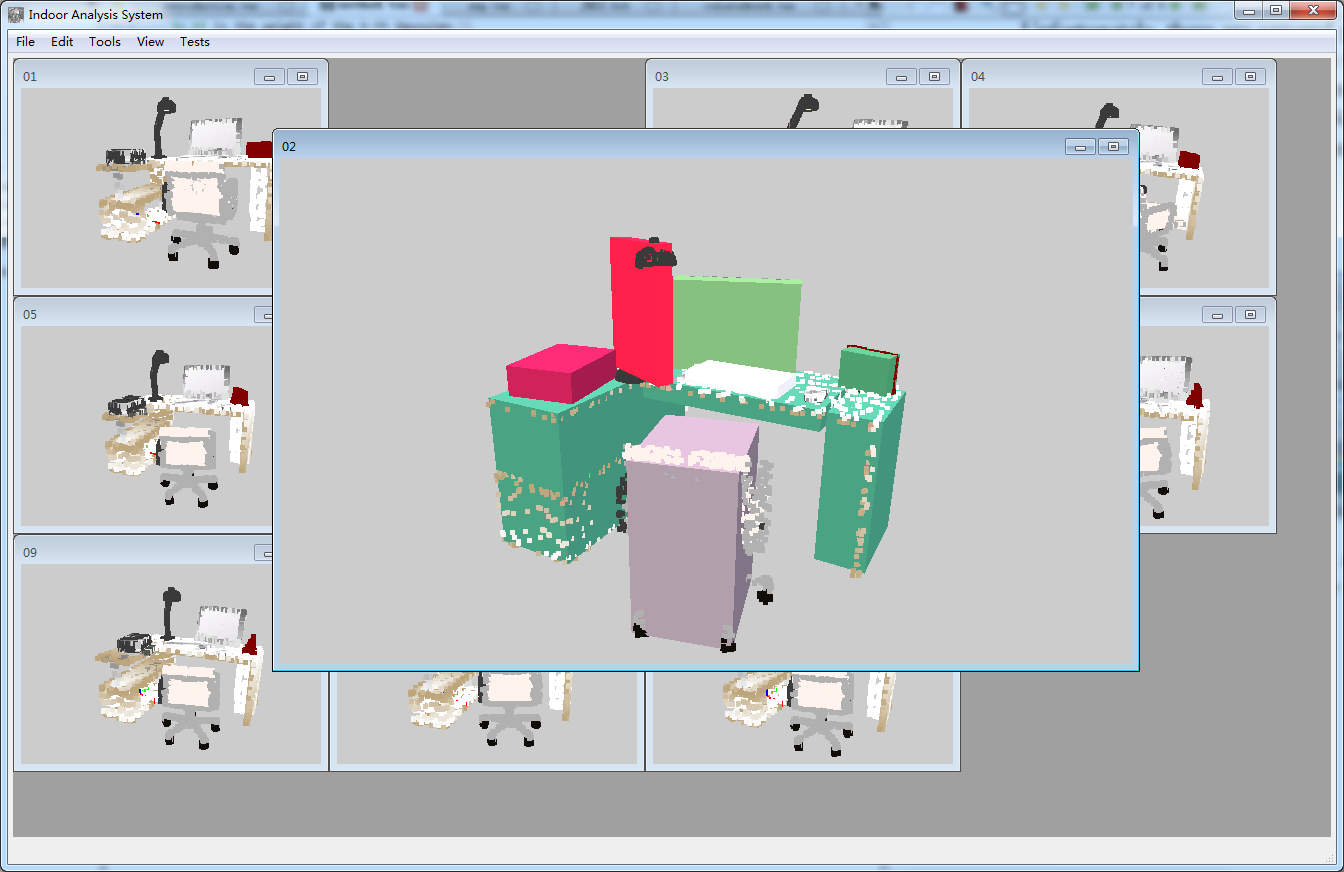
\includegraphics[width=.3\linewidth]{images/interact05.png}
	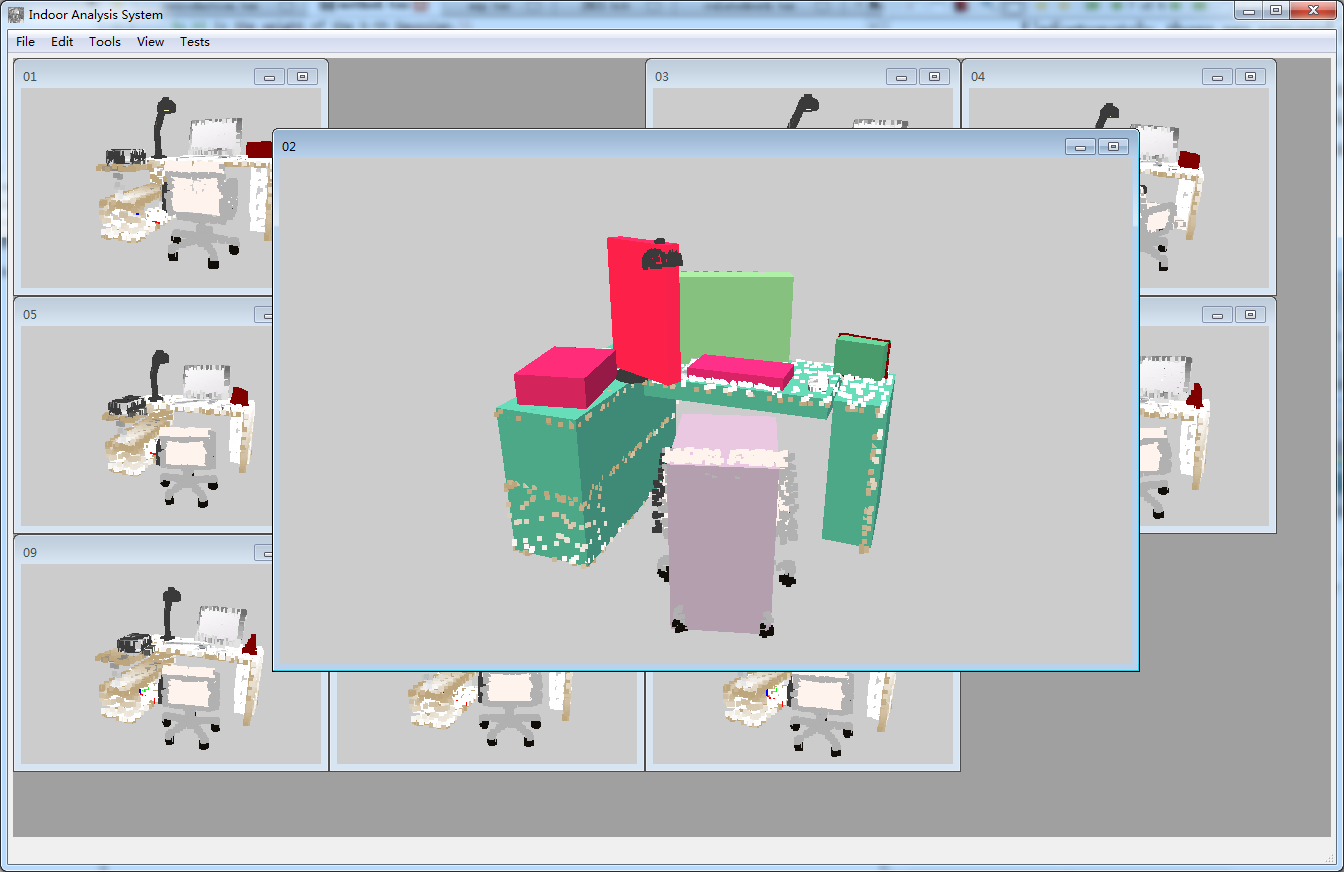
\includegraphics[width=.3\linewidth]{images/interact06.png}
	\caption{\label{fig:interact}
		From the first to the nineth, the nine images show the procedure of interaction:
		the user pick one point set and place boxes in it to indicate the layout for this point set. The box in white is the box currently under editing. The boxes in other colors are boxes placed to represent object layouts. One color represent one object. The interaction allows multiple boxes to represent same object.(e.g. the desk is represented by three boxes in same color)}
\end{figure}
These two paremeters are difficult to be initialized without semantic prior, but with the input of the users we can naturally initialize the $N$ as the number of different color label and the ${K_n}$ as 
\begin{equation}
K_n=\frac{V_n}{\sum V_n}K_{all}
\end{equation}
in which the $V_n$ represent the total volume of the boxes in the n-th color and the $K_{all}$ is initialized as $K_{all}=0.5*median(I_m)$ and $\{I_m\}$ are point numbers of $M$ input point set. This is an emperical choice borrowed from \cite{Evangelidis2014}.


